
\chapter*{Dev Notes}
WILL BE REMOVED

\section{Theory Check}

\subsection{Concrete AF}

\begin{center}
	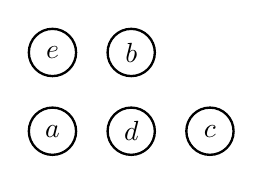
\begin{tikzpicture}
		\def \ax{0.0} \def \ay{-1.0}
		\def \bx{1.0} \def \by{0.0}
		\def \cx{2.0} \def \cy{-1.0}
		\def \dx{1.0} \def \dy{-1.0}
		\def \ex{0.0} \def \ey{0.0}
  
        % Singletons
        \draw[line width=0.3mm] (\ax,\ay)  circle (0.3) node[anchor=center]{$a$};
        \draw[line width=0.3mm] (\bx,\by)  circle (0.3) node[anchor=center]{$b$};
        \draw[line width=0.3mm] (\cx,\cy)  circle (0.3) node[anchor=center]{$c$};
        \draw[line width=0.3mm] (\dx,\dy)  circle (0.3) node[anchor=center]{$d$};
        \draw[line width=0.3mm] (\ex,\ey)  circle (0.3) node[anchor=center]{$e$};
		% Attacks
		\DrawAttackHorizontal{R}{\ex}{\ey}{\bx}{\by}
		\DrawAttackHorizontal{L}{\dx}{\dy}{\ax}{\ay}
		\DrawAttackHorizontal{R}{\dx}{\dy}{\cx}{\cy}

		\DrawAttackVertical{B}{\bx}{\by}{\dx}{\dy}
		\DrawSelfAttackRightSingleton{\bx}{\by}
		\DrawSelfAttackRightSingleton{\cx}{\cy}
        
	\end{tikzpicture}
\end{center}
\textbf{Stable Sets:} $\{ d, e\}$

\subsection{Abstract AF}
\begin{center}
	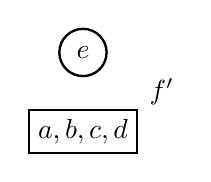
\begin{tikzpicture}
		\def \ex{0.0} \def \ey{ 0.0}
		\def \fx{0.0} \def \fy{-1.0}
        % Clusters
        \node[rectangle, draw, line width=0.3mm] at (\fx, \fy) {$a,b,c,d$};
		\node at (1, -0.5) {$f'$};
        % Singletons
        \draw[line width=0.3mm] (\ex,\ey)  circle (0.3) node[anchor=center]{$e$};
		% Attacks
		\DrawAttackVertical{D}{\ex}{\ey}{\fx}{\fy}
		\DrawSelfAttackLeftTopCluster{\fx-0.63}{\fy + 0.3}
	\end{tikzpicture}
\end{center}
\textbf{Stable Sets:} $\{ f', e\}$, $\{ e\}$

Abstract AF is \textbf{spurious} to concrete AF because set $\{ e\}$.



\subsection{Concretized AF (b,d) Grounded}
\begin{center}
	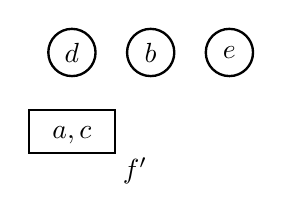
\begin{tikzpicture}
		\def \bx{1.0} \def \by{0.0}
		\def \dx{0.0} \def \dy{0.0}
		\def \ex{2.0} \def \ey{0}
		\def \fx{0.0} \def \fy{-1.0}
        % Clusters
        \node[rectangle, draw, line width=0.3mm] at (\fx, \fy) {$\phantom{d}a, c\phantom{d}$};
		\node at (0.8, -1.5) {$f'$};
        % Singletons
        \draw[line width=0.3mm] (\bx,\by)  circle (0.3) node[anchor=center]{$b$};
        \draw[line width=0.3mm] (\dx,\dy)  circle (0.3) node[anchor=center]{$d$};
        \draw[line width=0.3mm] (\ex,\ey)  circle (0.3) node[anchor=center]{$e$};
		% Attacks
		\DrawAttackHorizontal{B}{\bx}{\by}{\dx}{\dy}
		\DrawAttackHorizontal{L}{\ex}{\ey}{\bx}{\by}

		\DrawAttackVertical{D}{\dx}{\dy}{\fx}{\fy}

		\DrawSelfAttackRightSingleton{\bx}{\by}

		\DrawSelfAttackLeftTopCluster{\fx-0.45}{\fy + 0.3}
        
	\end{tikzpicture}
\end{center}
\textbf{Stable Sets:} $\{ d, e\}$, $\{ d, e, f'\}$

Concretized AF (b, d) is \textbf{spurious} to concrete AF because set $\{ d, e, f'\}$.


\subsection{Concretized AF (b)}
\begin{center}
	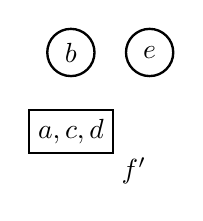
\begin{tikzpicture}
		\def \bx{0.0} \def \by{ 0.0}
		\def \ex{1.0} \def \ey{ 0.0}
		\def \fx{0.0} \def \fy{-1.0}
        % Clusters
        \node[rectangle, draw, line width=0.3mm] at (\fx, \fy) {$a,c,d$};
		\node at (0.8, -1.5) {$f'$};
        % Singletons
        \draw[line width=0.3mm] (\bx,\by)  circle (0.3) node[anchor=center]{$b$};
        \draw[line width=0.3mm] (\ex,\ey)  circle (0.3) node[anchor=center]{$e$};
		% Attacks
		\DrawAttackHorizontal{L}{\ex}{\ey}{\bx}{\by}
		\DrawAttackVertical{B}{\bx}{\by}{\fx}{\fy}

		\DrawSelfAttackRightSingleton{\bx}{\by}

		\DrawSelfAttackLeftTopCluster{\fx-0.45}{\fy + 0.3}
	\end{tikzpicture}
\end{center}
\textbf{Stable Sets:} $\{ f', e\}$

Concretized AF (e) is \textbf{faithful} to concrete AF.



\newpage
\section{Problem of Concretization Combinations}
\subsection{Concrete AF}
Let $X=(ARG, ATT)$ be a concrete AF with the following arguments and attacks. Then the stable sets $stb(X)$ would be $\{\}, \{a,b,d,f\}, \{b,c,d,g\}$.
\begin{center}
	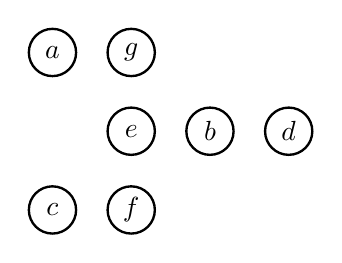
\begin{tikzpicture}
		\def \ax{0} \def \ay{0}
		\def \bx{2} \def \by{-1}
		\def \cx{0} \def \cy{-2}
		\def \dx{3} \def \dy{-1}
		\def \ex{1} \def \ey{-1}
		\def \fx{1} \def \fy{-2}
		\def \gx{1} \def \gy{0}

		% Singletons
		\draw[line width=0.3mm] (\ax,\ay)  circle (0.3) node[anchor=center]{$a$};
		\draw[line width=0.3mm] (\bx,\by)  circle (0.3) node[anchor=center]{$b$};
		\draw[line width=0.3mm] (\cx,\cy)  circle (0.3) node[anchor=center]{$c$};
		\draw[line width=0.3mm] (\dx,\dy)  circle (0.3) node[anchor=center]{$d$};
		\draw[line width=0.3mm] (\ex,\ey)  circle (0.3) node[anchor=center]{$e$};
		\draw[line width=0.3mm] (\fx,\fy)  circle (0.3) node[anchor=center]{$f$};
		\draw[line width=0.3mm] (\gx,\gy)  circle (0.3) node[anchor=center]{$g$};
		% Attacks
		\DrawAttackHorizontal{R}{\ax}{\ay}{\gx}{\gy}
		\DrawAttackHorizontal{R}{\cx}{\cy}{\fx}{\fy}
		\DrawAttackVertical{B}{\ax}{\ay}{\cx}{\cy}
		\DrawAttackDiagonal{NLR}{\ax}{\ay}{\ex}{\ey}
		\DrawAttackVertical{D}{\gx}{\gy}{\ex}{\ey}
	\end{tikzpicture}
\end{center}

\subsection{Abstract AF}
If we now abstract the concrete AF $X$ to $X'$, we obtain the following stable sets $\{\}, \{h'\}, \{h', g\}, \{g\}$.
This would lead to a spurious abstraction, due to set $\{g\}$.
\begin{center}
	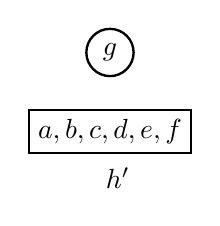
\begin{tikzpicture}
		\def \gx{0} \def \gy{0}
		\def \hx{0} \def \hy{-1}

		% Cluster
		\node[rectangle, draw, line width=0.3mm] at (\hx, \hy) {$a,b,c,d,e,f$};
		\node at (0.1, -1.6) {$h'$};
		% Singletons
		\draw[line width=0.3mm] (\gx,\gy)  circle (0.3) node[anchor=center]{$g$};
		% Attacks
		\DrawAttackVertical{U}{\hx}{\hy}{\gx}{\gy}
		\DrawSelfAttackLeftTopCluster{\hx - 1}{\hy + 0.3}
	\end{tikzpicture}
\end{center}
Now let $X'$ be the input to our \texttt{CONCRETIZER} program and we parse as concretizer list the argument $f$.

\subsection{Concretized Abstract AF (f)}
We obtain the following AF $X''$ with the following stable sets $\{\}$, $\{h'\}$, $\{f, g, h'\}$, $\{g, h'\}$, $\{f, h'\}$, $\{f, g\}$.
Which would lead to a spurious abstraction, due to the sets $\{h'\}$, $\{f, g, h'\}$, $\{f, g\}$.
\begin{center}
	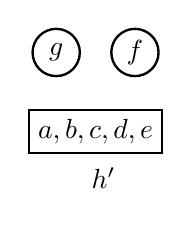
\begin{tikzpicture}
		\def \fx{0.5} \def \fy{0}
		\def \gx{-0.5} \def \gy{0}
		\def \hx{0} \def \hy{-1}

		% Cluster
		\node[rectangle, draw, line width=0.3mm] at (\hx, \hy) {$a,b,c,d,e$};
		\node at (0.1, -1.6) {$h'$};
		% Singletons
		\draw[line width=0.3mm] (\gx,\gy)  circle (0.3) node[anchor=center]{$g$};
		\draw[line width=0.3mm] (\fx,\fy)  circle (0.3) node[anchor=center]{$f$};
		% Attacks
		\DrawAttackVertical{U}{\hx + 0.5}{\hy}{\fx}{\fy}
		\DrawAttackVertical{U}{\hx - 0.5}{\hy}{\gx}{\gy}
		\DrawSelfAttackLeftTopCluster{\hx - 0.8}{\hy + 0.3}
	\end{tikzpicture}
\end{center}

\subsection{Concretizing until Faithfulness}
Since we want to obtain a faithful abstraction of the AF $X'$ with the concretized argument $f$, we create all possible combinations of further concretization.
Therefore, we need the spurious sets of $X''$ i.e. $\{h'\}$, $\{f, g, h'\}$, $\{f, g\}$. Since we are in the stable semantics, the depth of the concretizer search
is $2$ (i.e. if an argument $x$ is spurious, we investigate all its attackers, and the attacker of the attackers and the same for the defenders (=the arguments which $x$ attacks)).
\subsubsection{Pre Filtering}
The spurious sets of $X''$ can also have clusters in the sets. Since we relate to the attackers and defenders of the concrete AF $X$ we can filter them out (because the concrete
AF has no clusters). We then obtain the following sets: $\{f, g\}$, $\{f, g\}$, which can be reduced to $\{f, g\}$.
\subsubsection{Attacker and Defender Depth 2}
We now iterate over the filtered sets and check for each attacker $a$, the attackers of the attacker $a_x$. We also check, if $a$ or $a_x$ is in a cluster, because if they are not, we can not concretize them.
Furthermore we add all the elements $c$ from the concretizer list (if not already present) and create the following list of sets: $[\{a, c\}$, $\{a, a_0\, c\}$,  $\{a, a_1\, c\}$, $...$,  $\{a, a_n, c\}]$
which in the current example would lead to the following list: $[\{c, f\}, \{a, c, f\}, \{a, f, g\}, \{a, c, f, g\}]$.
The exact same is done with the defenders, where the list is $[\{e, f, g\}]$.
\subsubsection{Combining Sets}
\label{sssec:l}
We now create each possible combination out of the 5 lists. This leads to a total of $\sum_{k=1}^{5} {5 \choose k}=31$ solutions. Since f.e. the combination $\{c, f\}$ and and $\{a, c, f\}$ are already covered in $\{a, c, f\}$ we remove the duplicates and
obtain the following seven sets: $\{c, f\}$, $\{a, f\}$, $\{e, f\}$, $\{a, c, f\}$, $\{c, e, f\}$, $\{a, e, f\}$, $\{a, c, e, f\}$.

\section{Problem}
This approach works well for very small AF. But once we have more spurious sets, the list of the combinations ~\ref{sssec:l} grows vastly. I had one instance, were $11$ spurious sets led to $120$ combinations
which would then lead to  $\sum_{k=1}^{120} {120 \choose k}$ combinations, which is simply not feasible. Since conflict free sets produce a lot of sets, this case is not abstract and quite common.

\section{Thoughts}
If we consider the "larger" combinations first and once they result into faithfulness, we reduce the search to the selected set and try to concretize further each argument one by one. This would return a faithful solution.
But I am not sure if it holds, that if the "larger" concretization AF is spurious, its fragmentation has to be spurious as well.
To explain further what I mean: Let's take the previous example, where we tried to concretize the argument $f$.
\begin{center}
	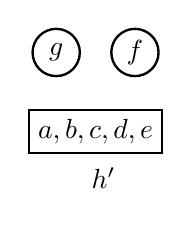
\begin{tikzpicture}
		\def \fx{0.5} \def \fy{0}
		\def \gx{-0.5} \def \gy{0}
		\def \hx{0} \def \hy{-1}

		% Cluster
		\node[rectangle, draw, line width=0.3mm] at (\hx, \hy) {$a,b,c,d,e$};
		\node at (0.1, -1.6) {$h'$};
		% Singletons
		\draw[line width=0.3mm] (\gx,\gy)  circle (0.3) node[anchor=center]{$g$};
		\draw[line width=0.3mm] (\fx,\fy)  circle (0.3) node[anchor=center]{$f$};
		% Attacks
		\DrawAttackVertical{U}{\hx + 0.5}{\hy}{\fx}{\fy}
		\DrawAttackVertical{U}{\hx - 0.5}{\hy}{\gx}{\gy}
		\DrawSelfAttackLeftTopCluster{\hx - 0.8}{\hy + 0.3}
	\end{tikzpicture}
\end{center}

Since this was spurious, we created the concretizer list $\{c, f\}$, $\{a, f\}$, $\{e, f\}$, $\{a, c, f\}$, $\{c, e, f\}$, $\{a, e, f\}$, $\{a, c, e, f\}$. Instead of creating the complete concretizer list (which is not feasible for a large number of solutions as explained before)
we produce a single set that contains all the unique singletons of the combinations, so in this example  $\{a, c, e, f\}$. This is faithful, so we focus only on this set and try to concretize its combinations. So in this case: $\{a, f\}$, $\{c, f\}$, $\{e, f\}$,  $\{a, c, f\}$, $\{a, e, f\}$, $\{c, e, f\}$. If one of these
is faithful, we found a better solution than the "larger" one. If all of these combinations are spurious, we just return the "larger" one.

For this approach I would simply compare each spurious solution, create one list of all the unique arguments. Instead of creating the combination list, I extend the spurious solution list with the attackers (and its attackers) and defenders (and its defenders).